\section[Theory]{Theory}
\label{sec:theory}

\begin{frame}{Bifurcations and Critical Slowing Down}
	\textbf{Bifurcation}: A qualitative change in the `motion' of a dynamical System due to a quantitative change in one of its parameters. Serious bifurcations, called \textcolor{red}{Critical Bifurcations}, cause the system to become unstable from stable.
\end{frame}

\begin{frame}{Bifurcations and Critical Slowing Down}
	\begin{figure}
		\centering
		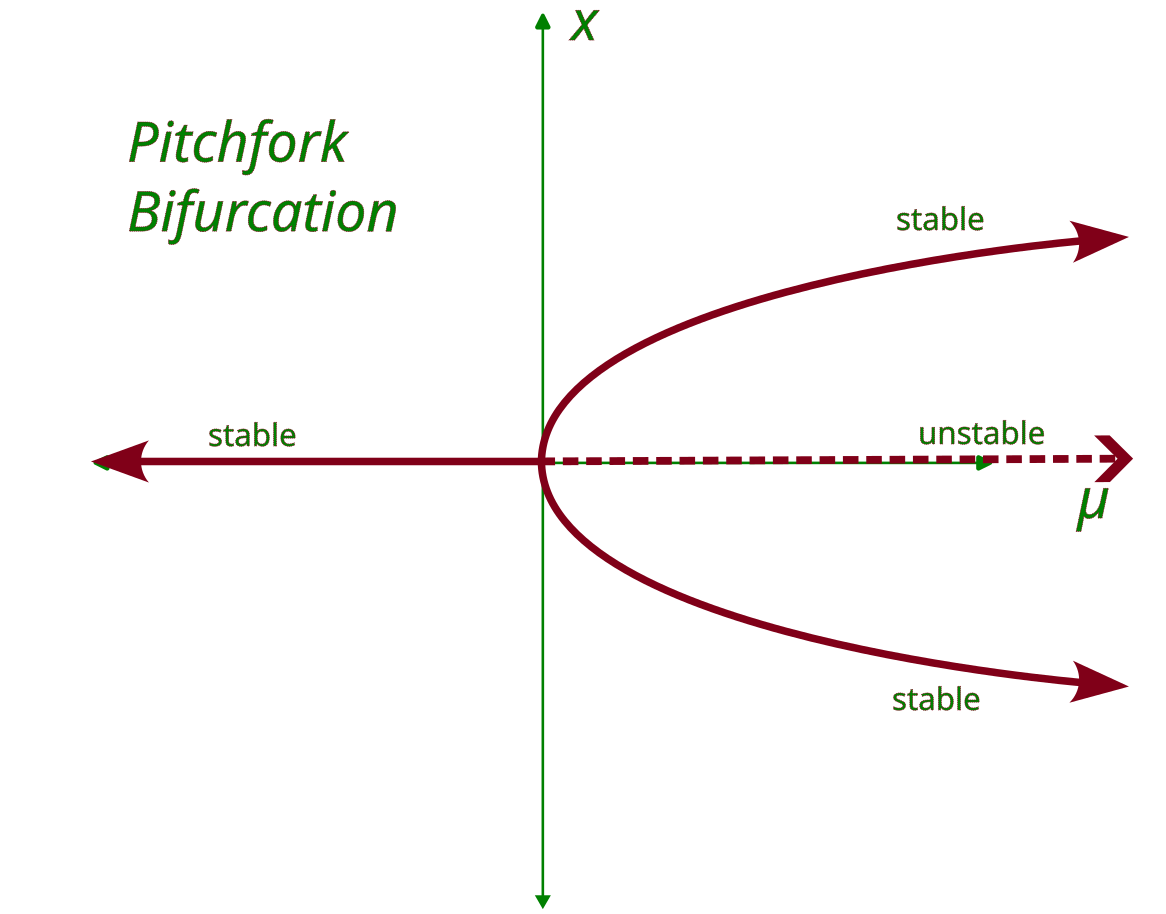
\includegraphics[scale=0.15]{../figures/bftrans1.png}
		\label{fig:transcritBifurcation}
		\caption{Bifurcation Diagram showing the Normal form of Pitchfork Bifurcation}
		\begin{equation}
			\frac{dx}{dt} = \mu x - x^3
		\end{equation}
	\end{figure}
\end{frame}

\begin{frame}{Bifurcations and Critical Slowing Down}
	\textbf{Critical Slowing Down}: Dynamical Systems exhibit early statistical warning signs before collapsing, i.e. before a critical bifurcation, they exhibit these signs:
	\begin{itemize}
		\item Increased recovery times from perturbations.
		\item Increased signal variance from the mean trajectory.
		\item Increased flicker and asymmetry in the signal
	\end{itemize}
	The above three properties can be identified by increasing variance and autocorrelation in time-series measurements taken from the system.
\end{frame}

\begin{frame}{AR1 and Variance}
	\begin{equation}
		\label{eq:autocorrDef}
		d[k] = a_1 d[k-1] + e[k]
	\end{equation} 
	Autoregressive Model of Order 1 on detrended voltages.
	
	\begin{equation}
		\label{eq:varDef}
		\sigma^2 = \frac{1}{n_k} \sum_{k=1}^{n_k} d[k]^2
	\end{equation} 
	Sample variance on detrended voltages.
\end{frame}